\documentclass[12pt]{article}
\usepackage[margin=1in]{geometry}

%\usepackage{pstricks,pst-node}
\usepackage{graphicx}
\usepackage{tikz}
\usetikzlibrary{automata,arrows}
\newcommand{\deriv}[1]{\ensuremath{\stackrel{#1}{\Longrightarrow}}}
\newcommand{\myfig}[1]{\includegraphics[scale=0.25]{figures/#1.png}}
\newcommand{\arr}[2]{$#1\rightarrow #2$}
\newcommand{\arrl}[1]{$#1\rightarrow \mt$}
\newcommand{\ar}{\rightarrow}
\newcommand{\mt}{\ensuremath{\epsilon}}

\title{Some simple LR parse tables}
\author{Geoffrey Matthews}
\begin{document}
\maketitle

\begin{description}

\item[Left recursion: $ S \rightarrow Sa\ |\ a$]\mbox{}\\

\begin{tabular}{lr}
Stack & Input \\
0 & a a a a \$ \\
0 a 1 & a a a \$ \\
0 S 2 & a a a \$ \\
0 S 2 a 3 & a a  \$ \\
0 S 2 & a a  \$ \\
0 S 2 a 3 & a  \$ \\
0 S 2 & a  \$ \\
0 S 2 a 3 &  \$ \\
0 S 2 & \$ \\
\end{tabular}
\hfill
\begin{tabular}{|c|c|c|c|}\hline
 & $a$ & \$ & $S$ \\\hline
0 & 1 & & 2\\\hline
1 & $S\rightarrow a$ &&\\\hline
2 & 3 & accept& \\\hline
3 & $S \rightarrow Sa$ & $S \rightarrow Sa$ &\\\hline
\end{tabular}

\hfill
\myfig{lrparseexamples01}


\pagebreak



\item[Right recursion:
$ S \rightarrow aS\ |\ a$]\mbox{}\\

\begin{tabular}{lr}
Stack & Input \\
0 & a a a a \$ \\
0 a 1 & a a a  \$ \\
0 a 1 a 1 & a a  \$ \\
0 a 1 a 1 a 1 & a  \$ \\
0 a 1 a 1 a 1 a 1 & \$ \\
0 a 1 a 1 a 1 S 2 & \$ \\
0 a 1 a 1 S 2 & \$ \\
0 a 1 S 2 & \$ \\
0 S 3 & \$ \\
\end{tabular}
\hfill
\begin{tabular}{|c|c|c|c|}\hline
 & $a$ & \$ & $S$ \\\hline
0 & 1 & & 3 \\\hline
1 & 1 & $S \rightarrow a$ & 2 \\\hline
2 & & $S\rightarrow aS$ & \\\hline
3 &  & accept & \\\hline
\end{tabular}

\hfill
\myfig{lrparseexamples02}


\newpage
\item[Middle recursion: $S \rightarrow aSa\ |\ bSb\ |\ c$]\mbox{}\\

\begin{tabular}{lr}
Stack & Input \\
0 & a b c b a \$ \\
0 a 1 & b c b a  \$ \\
0 a 1 b 2 & c b a  \$ \\
0 a 1 b 2 c 3 & b a  \$ \\
0 a 1 b 2 S 5 & b a  \$ \\
0 a 1 b 2 S 5 b 7 & a  \$ \\
0 a 1 S 4 & a  \$ \\
0 a 1 S 4 a 6 & \$ \\
0 S 8 & \$\\
\end{tabular}
\hfill
\begin{tabular}{|c|c|c|c|c|c|}\hline
 & a & b & c & \$ & S \\\hline
0 & 1 & 2 & 9 && 8\\\hline
1 & 1 & 2 & 3 && 4\\\hline
2 & 1 & 2 & 3 && 5\\\hline
3 & $S\rightarrow c$& $S\rightarrow c$&&&\\\hline
4 & 6 &&&&\\\hline
5 &&7&&&\\\hline
6 & $S\rightarrow aSa$ & $S\rightarrow aSa$ &&$S\rightarrow aSa$ &\\\hline
7 & $S\rightarrow bSb$ & $S\rightarrow bSb$ &&$S\rightarrow bSb$&\\\hline
8 &&&&accept&\\\hline
9 &&&&$S\rightarrow c$&\\\hline
\end{tabular}


\vspace{0.5in}

\myfig{lrparseexamples03}

\newpage
\item[Example: $a^*b^*b$]

\begin{eqnarray*}
S &\rightarrow& AB\\
A &\rightarrow& aA\ |\ \mt\\
B &\rightarrow& bB\ |\ b
\end{eqnarray*}

\begin{tabular}{lr}
Stack & Input \\
0 & a a b b b \$\\
0 a 1 & a b b b \$\\
0 a 1 a 1 & b b b \$\\
0 a 1 A 2 & b b b \$\\
0 A 3 & b b b  \$\\
0 A 3 b 4 &  b b \$\\
0 A 3 b 4 b 4 & b \$\\
0 A 3 b 4 b 4 b 4 & \$\\
0 A 3 b 4 b 4 B 5 & \$\\
0 A 3 b 4 B 5 &  \$\\
0 A 3 B 6 &  \$\\
0 S 7 & \$\\
\end{tabular}
\begin{tabular}{|c|c|c|c|c|c|c|}\hline
 & a & b & \$ & S & A & B \\\hline
0 & 1 & $A\rightarrow\mt$&&7&3&\\\hline
1 & 1 & $A\rightarrow\mt$&&&2&\\\hline
2 &&$A\rightarrow aA$&&&&\\\hline
3 &&4&&&&6\\\hline
4 &&4&$B\rightarrow b$&&&5\\\hline
5 &&&$B\rightarrow bB$&&&\\\hline
6 &&&$S\rightarrow AB$&&&\\\hline
7 &&&accept&&&\\\hline
\end{tabular}


\begin{tabular}{lr}
Stack & Input \\
0 & b b b \$\\
0 A 3 & b b b \$\\
0 A 3 b 4 & b b \$\\
0 A 3 b 4 b 4 & b \$\\
0 A 3 b 4 b 4  b 4 & \$\\
0 A 3 b 4 b 4  B 5 & \$\\
0 A 3 b 4 B 5 & \$\\
0 A 3 B 6 & \$\\
0 S 7 & \$\\
\end{tabular}
\myfig{lrparseexamples04}

\newpage
\item[Example: $a^mb^nc^{m+n}$, Part I]
\begin{eqnarray*}
S &\rightarrow& aSc \mid B \\
B &\rightarrow& bBc \mid  \mt
\end{eqnarray*}

$S \deriv{S\ar B} B \deriv{B \ar \mt} \mt$

\begin{tabular}{lrl}
  Stack & Input & Rule\\
  0 &  \$ & $B\ar \mt$ \\
  0 B 1 &  \$ & $S\ar B$\\
  0 S 2 & \$ \\
\end{tabular}
\hfill
\begin{tabular}{|c|c|c|c|c|c|c|} \hline
    & a & b & c & \$ & S & B \\\hline
  0 &   &   &   & $B\ar\mt$  &2&1 \\\hline
  1 &   &   &   & $S\ar B$  && \\\hline
  2 &    &   &   & accept  && \\\hline
\end{tabular}

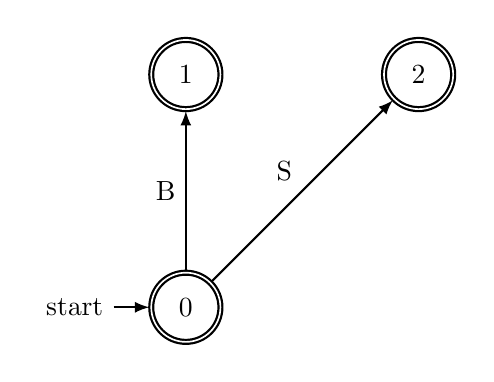
\begin{tikzpicture}[->,>=latex,thick,auto]
\matrix[row sep=2cm, column sep=2cm]{
  \node[state,accepting] (1) {1}; &
  \node[state,accepting] (2) {2}; \\
  \node[state,initial,accepting] (0) {0}; \\
  };
  \path (0) edge node {B} (1);
  \path (0) edge node {S} (2);
\end{tikzpicture}


\newpage
\item[Example: $a^mb^nc^{m+n}$, Part II]
\begin{eqnarray*}
S &\rightarrow& aSc \mid B \\
B &\rightarrow& bBc \mid  \mt
\end{eqnarray*}

$S \deriv{S\ar B} B \deriv{B \ar bBc} bBc \deriv{B\ar\mt} bc$

\begin{tabular}{lrl}
  Stack     & Input & Rule\\
  0         &  bc\$ & shift \\
  0 b 3     &   c\$ & $B\ar \mt$ \\
  0 b 3 B 4 &   c\$ & shift \\
  0 b 3 B 4 c 5 &   \$ & $B\ar bBc$ \\
  0 B 1 &   \$ & $S\ar B$ \\
  0 S 2 &   \$ & $S\ar B$ \\
\end{tabular}
\hfill
\begin{tabular}{|c|c|c|c|c|c|c|} \hline
    & a & b & c & \$ & S & B \\\hline
  0 &   & 3 &   & $B\ar\mt$ &2&1  \\\hline
  1 &   &   &   & $S\ar B$ &&  \\\hline
  2 &    &   &   & accept &&  \\\hline
  3 &    &   & $B\ar \mt$   & &&4   \\\hline
  4 &    &    &  5 &   && \\\hline
  5 &    &    &    & $B\ar bBc$ &&  \\\hline
\end{tabular}


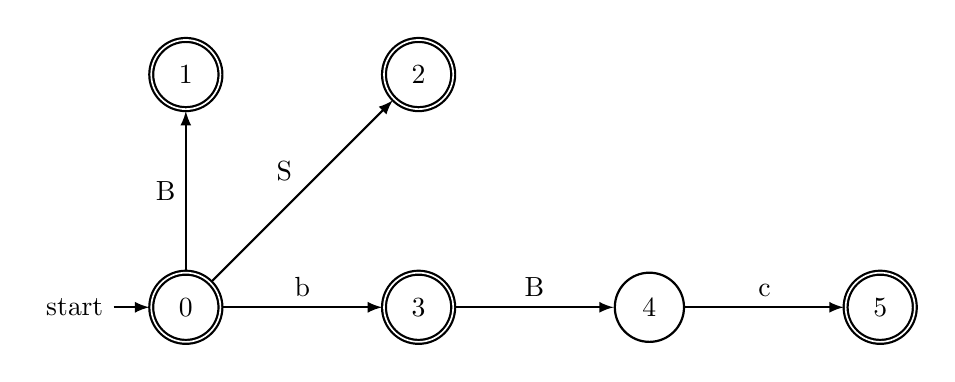
\begin{tikzpicture}[->,>=latex,thick,auto]
\matrix[row sep=2cm, column sep=2cm]{
  \node[state,accepting] (1) {1}; &
  \node[state,accepting] (2) {2}; \\
  \node[state,initial,accepting] (0) {0}; &
  \node[state,accepting] (3) {3}; &
  \node[state] (4) {4}; &
  \node[state,accepting] (5) {5};\\
  };
  \path (0) edge node {B} (1);
  \path (0) edge node {S} (2);
  \path (0) edge node {b} (3);
  \path (3) edge node {B} (4);
  \path (4) edge node {c} (5);
\end{tikzpicture}

\newpage
\item[Example: $a^mb^nc^{m+n}$, Part III]
\begin{eqnarray*}
S &\rightarrow& aSc \mid B \\
B &\rightarrow& bBc \mid  \mt
\end{eqnarray*}

$S \deriv{S\ar B} B \deriv{B \ar bBc} bBc \deriv{B\ar bBc} bbBcc \deriv{B\ar\mt} bbcc$

\begin{tabular}{lrl}
  Stack     & Input & Rule\\
  0         &  bbcc\$ & shift \\
  0 b 3     &   bcc\$ & shift \\
  0 b 3 b 3 &    cc\$ & $B\ar \mt$ \\
  0 b 3 b 3 B 4 &   cc\$ & shift \\
  0 b 3 b 3 B 4 c 5 & c\$ & $B\ar bBc$ \\
  0 b 3 B 4  &  c\$ & shift \\
  0 b 3 B 4 c 5 &  \$ &  $B\ar bBc$ \\
  0 B 1 &  \$ &  $S\ar B$ \\
  0 S 2 &   \$ & accept \\
\end{tabular}
\hfill
\begin{tabular}{|c|c|c|c|c|c|c|} \hline
    & a & b & c & \$ &S&B \\\hline
  0 &   & 3 &   & $B\ar\mt$ &2&1   \\\hline
  1 &   &   &   & $S\ar B$  && \\\hline
  2 &    &   &   & accept  && \\\hline
  3 &    & 3  & $B\ar \mt$   & && 4  \\\hline
  4 &    &    &  5 &   && \\\hline
  5 &    &    &   $B\ar bBc$  & $B\ar bBc$ &&  \\\hline
\end{tabular}


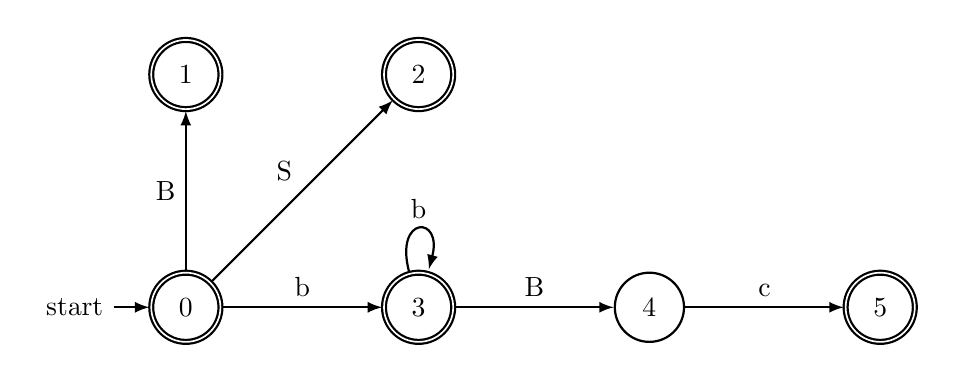
\begin{tikzpicture}[->,>=latex,thick,auto]
\matrix[row sep=2cm, column sep=2cm]{
  \node[state,accepting] (1) {1}; &
  \node[state,accepting] (2) {2}; \\
  \node[state,initial,accepting] (0) {0}; &
  \node[state,accepting] (3) {3}; &
  \node[state] (4) {4}; &
  \node[state,accepting] (5) {5};\\
  };
  \path (0) edge node {B} (1);
  \path (0) edge node {S} (2);
  \path (0) edge node {b} (3);
  \path (3) edge node {B} (4);
  \path (4) edge node {c} (5);
  \path (3) edge[loop above] node {b} (3);
\end{tikzpicture}

\newpage
\item[Example: $a^mb^nc^{m+n}$, Part IV]
\begin{eqnarray*}
S &\rightarrow& aSc \mid B \\
B &\rightarrow& bBc \mid  \mt
\end{eqnarray*}

$S \deriv{S\ar aSc} aSc
   \deriv{S\ar aSc} aaScc
   \deriv{S\ar B} aaBcc
   \deriv{B\ar\mt} aacc$

\begin{tabular}{lrl}
  Stack     & Input & Rule\\
  0         &  aacc\$ & shift \\
  0 a 6 &   acc\$ & shift \\
  0 a 6 a 6 &   cc\$ & $B\ar\mt$ \\
  0 a 6 a 6 B 7 &   cc\$ & $S\ar B$ \\
  0 a 6 a 6 S 8 &   cc\$ & shift \\
  0 a 6 a 6 S 8 c 9 &   c\$ & $S\ar aSc$ \\
  0 a 6 S 8         &   c\$ &  shift \\
  0 a 6 S 8 c 9     &   \$ & $S\ar aSc$ \\
  0 S 2     &   \$ & accept\\
\end{tabular}
\hfill
\begin{tabular}{|c|c|c|c|c|c|c|} \hline
    & a & b & c & \$ &S&B \\\hline
  0 & 6 & 3 &   & $B\ar\mt$ &2&1  \\\hline
  1 &   &   &   & $S\ar B$  && \\\hline
  2 &    &   &   & accept  && \\\hline
  3 &    & 3  & $B\ar \mt$   &  &&4  \\\hline
  4 &    &    &  5 &   && \\\hline
  5 &    &    &   $B\ar bBc$  & $B\ar bBc$ &&  \\\hline
  6 & 6  &    & $B\ar\mt$   &  && 7  \\\hline
  7 &    &    & $S\ar B$   &    &    &   \\\hline
  8 &    &    &  9  &    &    &   \\\hline
  9 &    &    &   $S\ar aSc$  &  $S\ar aSc$  &    &   \\\hline
\end{tabular}


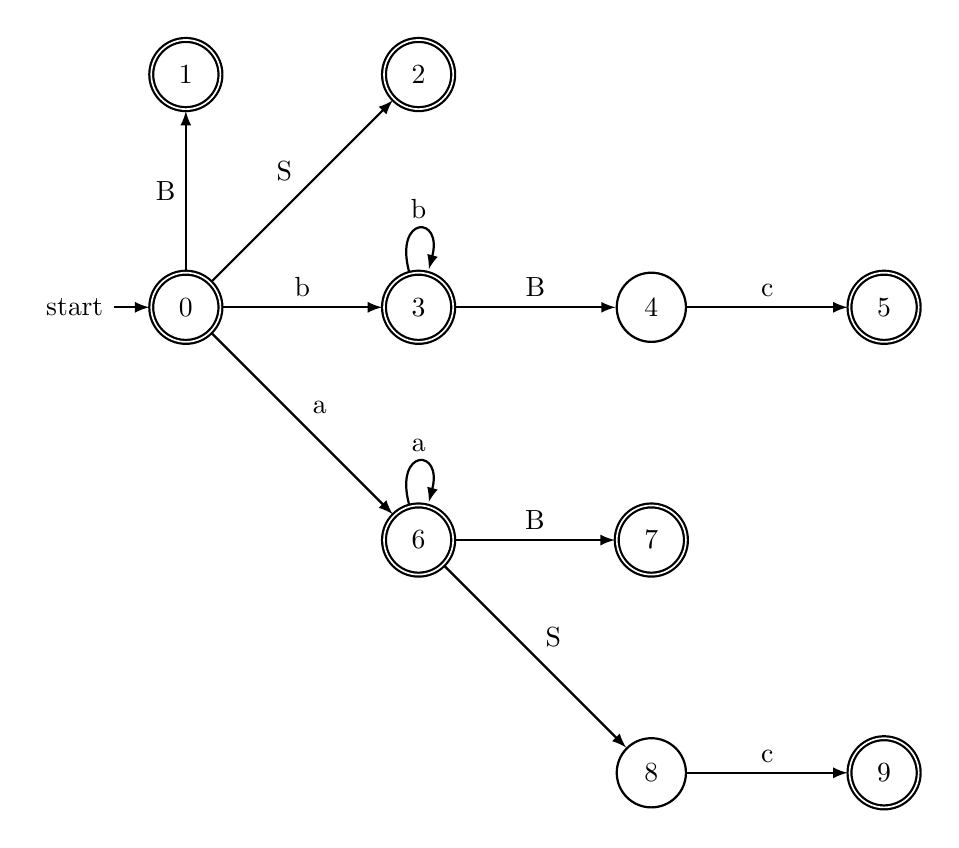
\begin{tikzpicture}[->,>=latex,thick,auto]
\matrix[row sep=2cm, column sep=2cm]{
  \node[state,accepting] (1) {1}; &
  \node[state,accepting] (2) {2}; \\
  \node[state,initial,accepting] (0) {0}; &
  \node[state,accepting] (3) {3}; &
  \node[state] (4) {4}; &
  \node[state,accepting] (5) {5};\\
  &
  \node[state,accepting] (6) {6}; &
  \node[state,accepting] (7) {7}; \\
  &&
  \node[state] (8) {8}; &
  \node[state,accepting] (9) {9};\\
};
\path (0) edge node {a} (6);
\path (6) edge [loop above] node {a} (6);
\path (6) edge node {B} (7);
\path (6) edge node {S} (8);
\path (8) edge node {c} (9);
\path (0) edge node {B} (1);
\path (0) edge node {S} (2);
\path (0) edge node {b} (3);
\path (3) edge node {B} (4);
\path (4) edge node {c} (5);
\path (3) edge[loop above] node {b} (3);
\end{tikzpicture}

\newpage
\item[Example: $a^mb^nc^{m+n}$, Part V]
   {\small
\begin{eqnarray*}
S &\rightarrow& aSc \mid B \\
B &\rightarrow& bBc \mid  \mt
\end{eqnarray*}

$S \deriv{S\ar aSc} aSc
   \deriv{S\ar aSc} aaScc
   \deriv{S\ar B} aaBcc
   \deriv{B\ar bBc} aabBccc
   \deriv{B\ar bBc} aabbBcccc
   \deriv{B\ar \mt} aabbcccc
$

   \hspace{-2cm}
     \begin{tabular}{lrl}
  Stack     & Input & Rule\\
  0         &  aabbcccc\$ & shift \\
  0 a 6 &   abbcccc\$ & shift \\
  0 a 6 a 6 &   bbcccc\$ & shift \\
  0 a 6 a 6 b 10 &   bcccc\$ & shift \\
  0 a 6 a 6 b 10 b 10&   cccc\$ & $B\ar\mt$ \\
  0 a 6 a 6 b 10 b 10 B 11&   cccc\$ & shift \\
  0 a 6 a 6 b 10 b 10 B 11 c 12 &   ccc\$ &$B\ar bBc$ \\
  0 a 6 a 6 b 10 B 11 &   ccc\$ &  shift \\
  0 a 6 a 6 b 10 B 11 c 12 &  cc\$& $B\ar bBc$ \\
  0 a 6 a 6 B 7 &  cc\$& $S\ar B$ \\
  0 a 6 a 6 S 8 &  cc\$& shift \\
  0 a 6 a 6 S 8 c 9 &  c\$& $S\ar aSc$ \\
  0 a 6 S 8 &  c\$& shift \\
  0 a 6 S 8 c 9 &  \$& $S\ar aSc$ \\
  0 S 2 &  \$& accept\\
     \end{tabular}
\hfill
\begin{tabular}{|c|c|c|c|c|c|c|} \hline
    & a & b & c & \$ &S&B \\\hline
  0 & 6 & 3 &   & $B\ar\mt$ &2&1  \\\hline
  1 &   &   &   & $S\ar B$  && \\\hline
  2 &    &    &   & accept  && \\\hline
  3 &    & 3  & $B\ar \mt$   &  &&4  \\\hline
  4 &    &    &  5 &   && \\\hline
  5 &    &    &   $B\ar bBc$  & $B\ar bBc$ &&  \\\hline
  6 & 6  & 10 & $B\ar\mt$   &  && 7  \\\hline
  7 &    &    & $S\ar B$   &    &    &   \\\hline
  8 &    &    &  9  &    &    &   \\\hline
  9 &    &    &   $S\ar aSc$  &  $S\ar aSc$  &    &   \\\hline
10 &     & 10 & $B\ar\mt$    &     &     & 11    \\\hline
11 &     &    &  12   &     &     &   \\\hline
12 &     &    &  $B\ar bBc$   &     &     &   \\\hline
\end{tabular}


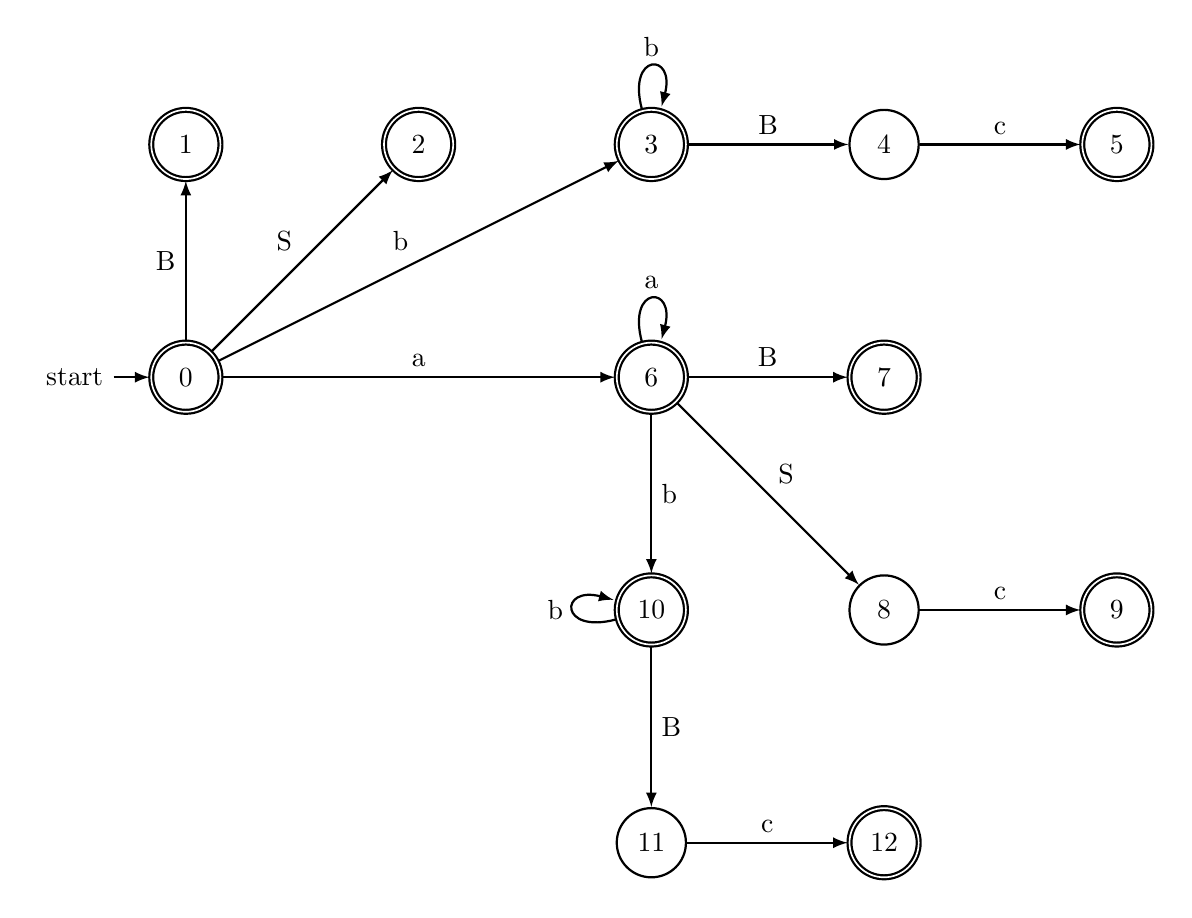
\begin{tikzpicture}[->,>=latex,thick,auto]
\matrix[row sep=2cm, column sep=2cm]{
  \node[state,accepting] (1) {1}; &
  \node[state,accepting] (2) {2}; &
  \node[state,accepting] (3) {3}; &
  \node[state] (4) {4}; &
  \node[state,accepting] (5) {5};\\
  \node[state,initial,accepting] (0) {0}; &&
  \node[state,accepting] (6) {6}; &
  \node[state,accepting] (7) {7}; \\
  &&
  \node[state,accepting] (10) {10}; &
  \node[state] (8) {8}; &
  \node[state,accepting] (9) {9};\\
  &&
  \node[state] (11) {11}; &
  \node[state,accepting] (12) {12};\\
};
\path (11) edge node {c} (12);
\path (10) edge node {B} (11);
\path (10) edge [loop left] node {b} (10);
\path (6) edge node {b} (10);
\path (0) edge node {a} (6);
\path (6) edge [loop above] node {a} (6);
\path (6) edge node {B} (7);
\path (6) edge node {S} (8);
\path (8) edge node {c} (9);
\path (0) edge node {B} (1);
\path (0) edge node {S} (2);
\path (0) edge node {b} (3);
\path (3) edge node {B} (4);
\path (4) edge node {c} (5);
\path (3) edge[loop above] node {b} (3);
\end{tikzpicture}

}

   Note that $(6,b)$ could jump to 3 instead of 10 and the graph
   would be simpler.
   
\newpage

\item[Same number of $a$s and $b$s, Part I]\mbox{}\\

\begin{eqnarray*}
S &\rightarrow&  \mt \mid aB |\ bA\\
A &\rightarrow& aS\ |\ bAA\\
B &\rightarrow& bS\ |\ aBB
\end{eqnarray*}


$S \Rightarrow \mt$\\\\
\begin{tabular}{lr}
Stack & Input \\
0     & \$\\
0 S 5 & \$\\
\end{tabular}\\\\
$S \Rightarrow aB \Rightarrow abS \Rightarrow ab$\\
\begin{tabular}{lr}
Stack & Input \\
0     & a b \$\\
0 a 1 b 2 & \$\\
0 a 1 b 2 S 3 & \$\\
0 a 1 B 4 & \$\\
0 S 5 & \$\\
\end{tabular}\hfill
\begin{tabular}{|c|c|c|c|c|c|c|}\hline
  & a & b & \$ & S & A & B \\\hline
0 & 1 &   & $S\ar \mt$   & 5  &   &   \\\hline
1 &   & 2 &    &   &   & 4  \\\hline
2 &   &   &\arrl{S}& 3  &   &   \\\hline
3 &   &   &\arr{B}{bS} &   &   &   \\\hline
4 &   &   &\arr{S}{aB} &   &   &   \\\hline
5 &   &   & accept &   &   &   \\\hline
\end{tabular}

\vspace{.5in}

\myfig{lrparseexamples05}


\newpage
\item[Same number of $a$s and $b$s, Part II]\mbox{}\\

\begin{eqnarray*}
S &\rightarrow& \mt \mid   aB |\ bA\\
A &\rightarrow& aS\ |\ bAA\\
B &\rightarrow& bS\ |\ aBB
\end{eqnarray*}

\centerline{$S \Rightarrow bA \Rightarrow baS \Rightarrow ba$}

\begin{tabular}{lr}
Stack & Input \\
0     & b a \$\\
0 b 6 & a \$\\
0 b 6 a 7 & \$\\
0 b 6 a 7 S 8 & \$\\
0 b 6 A 9 & \$\\
0 S 5 & \$\\
\end{tabular}\hfill
\begin{tabular}{|c|c|c|c|c|c|c|}\hline
  & a & b & \$ & S & A & B \\\hline
0 & 1 & 6 &    & 5  &   &   \\\hline
1 &   & 2 &    &   &   &  4 \\\hline
2 &   &   &\arrl{S}& 3 &   &   \\\hline
3 &   &   &\arr{B}{bS} &   &   &   \\\hline
4 &   &   &\arr{S}{aB} &   &   &   \\\hline
5 &   &   &  accept   &   &   &   \\\hline
6 & 7 &   &    &   & 9 &   \\\hline
7 &   &   &\arrl{S}& 8  &   &   \\\hline
8 &   &   &\arr{A}{aS} &   &   &   \\\hline
9 &   &   &\arr{S}{bA} &   &   &   \\\hline
\end{tabular}

\vspace{.5in}

\myfig{lrparseexamples06}



\newpage
\item[Same number of $a$s and $b$s, Part III]\mbox{}\\

\begin{eqnarray*}
S &\rightarrow&  \mt \mid  aB |\ bA\\
A &\rightarrow& aS\ |\ bAA\\
B &\rightarrow& bS\ |\ aBB
\end{eqnarray*}

\centerline{$S \Rightarrow aB\Rightarrow aaBB\Rightarrow aaBbS
\Rightarrow aaBb \Rightarrow aabSb \Rightarrow aabb$}

\begin{tabular}{lr}
Stack & Input \\
0     & a a b b \$\\
0 a 1 & a b b  \$\\
0 a 1 a 1 & b b  \$\\
0 a 1 a 1 b 2 & b  \$\\
0 a 1 a 1 b 2 S 3 & b \$\\
0 a 1 a 1 B 4 & b \$\\
0 a 1 a 1 B 4 b 10 &  \$\\
0 a 1 a 1 B 4 b 10 S 11 &  \$\\
\end{tabular}\hfill
\begin{tabular}{|c|c|c|c|c|c|c|}\hline
  & a & b & \$ & S & A & B \\\hline
0 & 1 & 6 &    & 5  &   &   \\\hline
1 & 1  & 2 &    &   &   &  4 \\\hline
2 &   &\arrl{S}&\arrl{S}& 3  &   &   \\\hline
3 &   &\arr{B}{bS}&\arr{B}{bS} &   &   &   \\\hline
4 &   & 10  &\arr{S}{aB} &   &   &   \\\hline
5 &   &   &  accept   &   &   &   \\\hline
6 & 7 &   &    &   & 9 &   \\\hline
7 &   &   &\arrl{S}& 8  &   &   \\\hline
8 &   &   &\arr{A}{aS} &   &   &   \\\hline
9 &   &   &\arr{S}{bA} &   &   &   \\\hline
10 &   &   &\arrl{S} & 11  &   &   \\\hline
11 &   &   &\arr{B}{bS} &   &   &   \\\hline
\end{tabular}

\vspace{.5in}

\myfig{lrparseexamples07}



\newpage
\item[Same number of $a$s and $b$s, Part IV]\mbox{}\\

\begin{eqnarray*}
S &\rightarrow&  \mt \mid  aB |\ bA\\
A &\rightarrow& aS\ |\ bAA\\
B &\rightarrow& bS\ |\ aBB
\end{eqnarray*}

\centerline{$S \Rightarrow aB\Rightarrow aaBB\Rightarrow aaBbS
\Rightarrow aaBb \Rightarrow aabSb \Rightarrow aabb$}

\begin{tabular}{lr}
Stack & Input \\
0     & a a b b \$\\
0 a 1 & a b b  \$\\
0 a 1 a 1 & b b  \$\\
0 a 1 a 1 b 2 & b  \$\\
0 a 1 a 1 b 2 S 3 & b \$\\
0 a 1 a 1 B 4 & b \$\\
0 a 1 a 1 B 4 b 2 &  \$\\
0 a 1 a 1 B 4 b 2 S 3 &  \$\\
\end{tabular}\hfill
\begin{tabular}{|c|c|c|c|c|c|c|}\hline
  & a & b & \$ & S & A & B \\\hline
0 & 1 & 6 &    & 5  &   &   \\\hline
1 & 1  & 2 &    &   &   & 4  \\\hline
2 &   &\arrl{S}&\arrl{S}& 3  &   &   \\\hline
3 &   &\arr{B}{bS}&\arr{B}{bS} &   &   &   \\\hline
4 &   & 2  &\arr{S}{aB} &   &   &   \\\hline
5 &   &   &  accept   &   &   &   \\\hline
6 & 7 &   &    &   & 9 &   \\\hline
7 &   &   &\arrl{S}& 8  &   &   \\\hline
8 &   &   &\arr{A}{aS} &   &   &   \\\hline
9 &   &   &\arr{S}{bA} &   &   &   \\\hline
\end{tabular}

\vspace{.5in}

\myfig{lrparseexamples08}

\newpage  \item[Same number of $a$s and $b$s, Part V]\mbox{}\\

\begin{eqnarray*}
S &\rightarrow&  \mt \mid  aB |\ bA\\
A &\rightarrow& aS\ |\ bAA\\
B &\rightarrow& bS\ |\ aBB
\end{eqnarray*}

\centerline{$S \Rightarrow aB\Rightarrow aaBB\Rightarrow aaBbS
\Rightarrow aaBb \Rightarrow aabSb \Rightarrow aabb$}

\begin{tabular}{lr}
Stack & Input \\
0     & a a b b \$\\
0 a 1 & a b b  \$\\
0 a 1 a 1 & b b  \$\\
0 a 1 a 1 b 2 & b  \$\\
0 a 1 a 1 b 2 S 3 & b \$\\
0 a 1 a 1 B 4 & b \$\\
0 a 1 a 1 B 4 b 2 &  \$\\
0 a 1 a 1 B 4 b 2 S 3 &  \$\\
0 a 1 a 1 B 4 B 10 &  \$\\
\end{tabular}\hfill
\begin{tabular}{|c|c|c|c|c|c|c|}\hline
  & a & b & \$ & S & A & B \\\hline
0 & 1 & 6 &    & 5  &   &   \\\hline
1 & 1  & 2 &    &   &   & 4  \\\hline
2 &   &\arrl{S}&\arrl{S}& 3  &   &   \\\hline
3 &   &\arr{B}{bS}&\arr{B}{bS} &   &   &   \\\hline
4 &   & 2  &\arr{S}{aB} &   &   &  10 \\\hline
5 &   &   &  accept   &   &   &   \\\hline
6 & 7 &   &    &   & 9 &   \\\hline
7 &   &   &\arrl{S}& 8  &   &   \\\hline
8 &   &   &\arr{A}{aS} &   &   &   \\\hline
9 &   &   &\arr{S}{bA} &   &   &   \\\hline
10 &   &   &\arr{B}{aBB} &   &   &   \\\hline
\end{tabular}

\vspace{.5in}

\myfig{lrparseexamples09}


\newpage  \item[Same number of $a$s and $b$s, Part VI]\mbox{}\\

\begin{eqnarray*}
S &\rightarrow&  \mt \mid  aB |\ bA\\
A &\rightarrow& aS\ |\ bAA\\
B &\rightarrow& bS\ |\ aBB
\end{eqnarray*}

\centerline{$S \Rightarrow aB\Rightarrow aaBB\Rightarrow aaBbS
\Rightarrow aaBb \Rightarrow aabSb \Rightarrow aabb$}

\begin{tabular}{lr}
Stack & Input \\
0     & a a b b \$\\
0 a 1 & a b b  \$\\
0 a 1 a 1 & b b  \$\\
0 a 1 a 1 b 2 & b  \$\\
0 a 1 a 1 b 2 S 3 & b \$\\
0 a 1 a 1 B 4 & b \$\\
0 a 1 a 1 B 4 b 2 &  \$\\
0 a 1 a 1 B 4 b 2 S 3 &  \$\\
0 a 1 a 1 B 4 B 10 &  \$\\
0 a 1 B 4 &  \$\\
0 S 5 &  \$\\
\end{tabular}\hfill
\begin{tabular}{|c|c|c|c|c|c|c|}\hline
  & a & b & \$ & S & A & B \\\hline
0 & 1 & 6 &    & 5  &   &   \\\hline
1 & 1  & 2 &    &   &   & 4  \\\hline
2 &   &\arrl{S}&\arrl{S}& 3  &   &   \\\hline
3 &   &\arr{B}{bS}&\arr{B}{bS} &   &   &   \\\hline
4 &   & 2  &\arr{S}{aB} &   &   &  10 \\\hline
5 &   &   &  accept   &   &   &   \\\hline
6 & 7 &   &    &   & 9 &   \\\hline
7 &   &   &\arrl{S}& 8  &   &   \\\hline
8 &   &   &\arr{A}{aS} &   &   &   \\\hline
9 &   &   &\arr{S}{bA} &   &   &   \\\hline
10 &   &   &\arr{B}{aBB} &   &   &   \\\hline
\end{tabular}

\vspace{.5in}

\myfig{lrparseexamples10}



\newpage  \item[Same number of $a$s and $b$s, Part VII]\mbox{}\\

\begin{eqnarray*}
S &\rightarrow&  \mt \mid  aB |\ bA\\
A &\rightarrow& aS\ |\ bAA\\
B &\rightarrow& bS\ |\ aBB
\end{eqnarray*}

\centerline{$S \Rightarrow bA \Rightarrow bbAA
\Rightarrow bbAaS \Rightarrow bbAa
\Rightarrow bbaSa \Rightarrow bbaa$}

\begin{tabular}{lr}
Stack & Input \\
0     & b b a a \$\\
0 b 6 &  b a a \$\\
0 b 6 b 6 & a a \$\\
0 b 6 b 6 a 7 & a \$\\
0 b 6 b 6 a 7 S 8 & a \$\\
0 b 6 b 6 A 9 & a \$\\
0 b 6 b 6 A 9 a 7 & \$\\
0 b 6 b 6 A 9 a 7 S 8 & \$\\
0 b 6 b 6 A 9 A 11 & \$\\
0 b 6 A 9 & \$\\
0 S 5 & \$\\
\end{tabular}\hfill
\begin{tabular}{|c|c|c|c|c|c|c|}\hline
  & a & b & \$ & S & A & B \\\hline
0 & 1 & 6 &    & 5  &   &   \\\hline
1 & 1  & 2 &    &   &   & 4  \\\hline
2 &   &\arrl{S}&\arrl{S}& 3  &   &   \\\hline
3 &   &\arr{B}{bS}&\arr{B}{bS} &   &   &   \\\hline
4 &   & 2  &\arr{S}{aB} &   &   &  10 \\\hline
5 &   &   &  accept   &   &   &   \\\hline
6 & 7 &   &    &   & 9 &   \\\hline
7 & \arrl{S} &   &\arrl{S}& 8  &   &   \\\hline
8 & \arr{A}{aS}  &   &\arr{A}{aS} &   &   &   \\\hline
9 & 7  &   &\arr{S}{bA} &   &   &   \\\hline
10 &   &   &\arr{B}{aBB} &   &   &   \\\hline
11 &   &   & \arr{A}{bAA}  &   &   &   \\\hline
\end{tabular}

\vspace{.5in}
By symmetry:

\myfig{lrparseexamples11}
\end{description}


\end{document}
